\documentclass[twoside]{article}
\usepackage{aistats2016}

% If your paper is accepted, change the options for the package
% aistats2016 as follows:
%
%\usepackage[accepted]{aistats2016}
%
% This option will print headings for the title of your paper and
% headings for the authors names, plus a copyright note at the end of
% the first column of the first page.


\begin{document}

% If your paper is accepted and the title of your paper is very long,
% the style will print as headings an error message. Use the following
% command to supply a shorter title of your paper so that it can be
% used as headings.
%
%\runningtitle{I use this title instead because the last one was very long}

% If your paper is accepted and the number of authors is large, the
% style will print as headings an error message. Use the following
% command to supply a shorter version of the authors names so that
% they can be used as headings (for example, use only the surnames)
%
%\runningauthor{Surname 1, Surname 2, Surname 3, ...., Surname n}

\twocolumn[

\aistatstitle{Extended and Unscented Kitchen Sinks}

\aistatsauthor{ Anonymous Author 1 \And Anonymous Author 2 \And Anonymous Author 3 }

\aistatsaddress{ Unknown Institution 1 \And Unknown Institution 2 \And Unknown Institution 3 } ]

 \begin{abstract}

    In this paper we propose a scalable multiple-output generalization of
    unscented and extended Gaussian processes. These algorithms have been
    designed to incorporate general nonlinear transformations in their
    likelihood functions by linearizing them using a Taylor series or the
    Unscented Transform in a variational inference framework, in which we also
    optimise all model parameters and hyperparameters. We achieve scalability
    by using random feature approximations of Gaussian process covariance
    functions, such as Random Kitchen Sink kernel approximations. We compare
    the new generalized algorithms on the same datasets as the original
    single-task algorithms. We also demonstrate the new algorithms classifying
    MNIST digits -- a task too large for the original algorithms, and
    performing a seismic inversion to infer the subsurface geological
    structures -- which is inherently a multi-task problem.

\end{abstract}

\section{Introduction}
% 
%In this paper we are interested in inference in models with Gaussian process (\gp)
%priors and  general (non-linear) likelihoods. 

Gaussian process models can be used as   
nonparametric probabilistic approaches to standard machine learning settings such as 
regression and classification \cite{rasmussen-williams-book}. For example, 
in classification problems  one places a  \gp prior over  latent functions, 
which are squashed through a likelihood model (such as a softmax or probit model)
in order to accurately represent the \emph{observable} targets.  
Therefore, in these situations, the latent functions in \gp-based models 
are nuisance parameters 
and are important only as a means to an end, i.e.~that of providing greater flexibility 
than their parametric counterparts.
  
In other applications in areas such as the natural and Earth sciences, the latent functions 
are quantities of interest themselves,  and they  
are passed through a domain-specific \emph{forward model}
in order to generate the observations.  As knowledge of the forward mapping from 
latent functions to the observations is available, but not the converse mapping, these
applications where reasoning about the latent functions is as important as 
the purely predictive setting, are usually referred to as \emph{inversion} problems. 

For example, in a geophysical inversion one might be interested in inferring rock 
properties (such as wave velocities) 
and the structural geometry of the  region   (such as boundaries between 
different types of formations) from geophysical data (such as wave travel times). 
There are strong constraints on how the latent functions (e.g.~rock properties) relate
 to the given observations, and these constraints are implemented in the forward model. 
 Clearly, in these types of applications, the goal is not only making good probabilistic predictions of the 
 observables but also having good estimates of the posterior over  the latent functions.

Both applications mentioned above,  standard machine learning tasks and inversion problems, 
present three key modeling and inference challenges when having Gaussian process (\gp) priors. 
The first challenge is scalability, as \gp{s} are notorious for their poor scalability as a function 
of the number of training points. The second challenge is multi-output and multi-task task learning, 
as required by problems such as multi-output regression, multi-class classification 
or inversion over a multi-layer geological structure (where each layer is a task). 
Finally, the  third challenge is that of dealing with non-linear likelihoods, for example 
in classification, regression with non-Gaussian noise, and seismic inversion,
 as the posterior over the latent functions is analytically intractable.  

In order to address these challenges, we build upon the work of  
\citet{steinberg-bonilla-nips-2014} who showed that it is possible to obtain
good posterior estimates, in models with Gaussian process priors and 
nonlinear likelihoods, using  approximations of the nonlinear  likelihood  
via a Taylor series expansion or via the Unscented Transform \citep{Julier2004}. 
They refer to the two  flavors of their approach as the 
extended Gaussian process (\egp) and the unscented Gaussian process (\ugp).
One of the fundamental reasons why such linearizations are effective is 
because of their locality and adaptivity, as they are 
constructed around the current posterior estimate, 
which is iteratively updated within a variational inference procedure.

While the method of \citet{steinberg-bonilla-nips-2014} is an
effective way to tackle nonlinearities in the likelihood, their approach  
does not deal with the other two challenges mentioned above, namely multi-task learning 
and scalability. Indeed their method is specific to single-output problems and 
inherits the cubic scalability of standard \gp models as a function of the number of 
training points. This scalability problem is exacerbated when formulating  multi-task 
our multiple-output settings, as  naively with $N$ data points and $M$ tasks their
computational cost would be $N^3M^3$ in time, 
which renders their approach impractical to large datasets.  

In this paper we propose a scalable multiple-output generalization  
of the method of \citet{steinberg-bonilla-nips-2014}.
We deal with multiple-output problems  by using 
affine transformations of the latent functions and 
achieve scalability by introducing random feature approximations 
 of the covariance function of the Gaussian processes, in the style of 
  \citet{rahimi-recht-nips-2007}, 
 all embedded into a variational inference framework. Since 
\citet{rahimi-recht-nips-2007} refer to their approach as 
Random Kitchen Sinks,  we will refer to our methods 
as extended and unscented kitchen sinks, when using 
the Taylor series approximation or the Unscented Transform approximation 
in the conditional likelihood respectively. 

Our approach naturally avoids the cubic scalability of the 
original \egp and \ugp methods \citep{steinberg-bonilla-nips-2014} as a function of the number 
of training points, with the complexity dominated by 
the inverse of the feature covariance of size $D$, which has a time complexity of
$\bigO(D^3)$. 

Our experiments, on small-scale synthetic nonlinear regression tasks and on 
a classification task on the \usps dataset, show that random feature approximations to the 
\egp and the \ugp can attain similar performance to the original methods, 
even when using a small number of features, hence reducing the complexity 
of inference significantly. Furthermore, experiments at a larger scale on 
the \mnist dataset, show that our algorithms are competitive with recently developed 
approaches for inference in \gp models, while the application of the \egp and \ugp to
this task is simply unfeasible. Finally, on a multi-task (joint) nonlinear seismic inversion  problem,
we show that our algorithms can recover accurate representations of the underlying 
geological structure and rock properties (seismic velocities) on simulated and real data.


\fix{TODO: need a couple more citations in the intro}
\fix{Discuss that people haven't actually evaluated the full posterior estimation using \rks approaches }

\fix{cite Andrew Wilson}
 



 







\section{GAUSSIAN PROCESS MODELS}
We are given $N$ input data points $ \{ \ins_n  \} \in \real{d}$ and their corresponding  
targets $\{ \outs_n  \} \in \real{P}$, which will  we describe compactly with $\cbrac{\Ins, \Outs}$,
where $\Ins \in \real{N \times d}$  and $\Outs \in \real{N \times P}$. Our goal is 
to learn a probabilistic mapping from inputs to outputs, which can be achieved through $Q$ latent  functions $\{ f_q \}$ and a given non-linear forward model $\nonlinf : \real{Q} \to \real{P}$. Additionally, we are interested in estimating the posterior over the latent functions given the observed data. 
While the former problem  is the standard multi-task supervised learning setting, we refer 
to the latter  as a probabilistic joint inversion problem, as we are given a forward mapping from 
latent functions to noiseless outputs but not the reverse. 

A fairly flexible modeling approach places independent zero-mean Gaussian process (GP) priors over 
the latent functions $\{ f_q \}$ with covariance functions $\kernel_q(\cdot, \cdot)$ and assumes iid observations given these latent functions. When these function are realized at the training data,
we obtain the following prior and likelihood models:
\begin{align}
	p(\latents)  &=  \prod_{q=1}^{Q} \Normal(\latentsq; \vec{0}, \KERNL_q) \\
	p(\outs | \latents) &= \prod_{n=1}^N p(\outs_n | \nonlinf ( \latentsn )) \text{,}
\end{align}
where $\KERNL_q$ is the covariance matrix induced by evaluating  the covariance 
function $\kernel_q$ at all input data $\Ins$; $\latentsq$ are  the values 
corresponding to latent function $q$ at all training inputs; 
and $\latentsn$ are  the values corresponding to all latent functions at input $\ins_n$. 

From a probabilistic inference perspective, solving the inversion problem (and the 
subsequent prediction problem), boils down to computing the posterior distribution 
$p(\latents | \Ins, \Outs)$. Unfortunately, this posterior distribution is, in general, 
intractable due to the non-linearities in $\nonlinf$, and one must resort to approximations.
%
\subsection{Variational Inference in Linearized GP Models}
\citet{steinberg-bonilla-nips-2014} have recently proposed a variational inference algorithm that
addresses the above inference problem for single output observations ($Q=1$).  
Such an algorithm relies upon the linearization of the forward model around the posterior 
mean, allowing for an analytic approximation of the evidence lower bound, which in turns 
enables the optimization of the variational parameters and hyperparameters within a simple 
but effective optimization procedure.  

To build such linearizations they use a Taylor series approximation and the unscented transform 
and, consequently, they refer to their methods to as the Extended Gaussian Process (\egp) and 
the Unscented Gaussian process (\ugp). 
The main advantage of their algorithms is that the linear
approximation is local and adaptive, as it is constructed around the posterior mean for a
single data point $n$, and it gets updated at every iteration of the algorithm as a function
of the variational parameters. 

However, such algorithms have the fundamental problem of poor scalability, as they 
inherit the computational cost of traditional GP models, which is $\calO(N^3)$. This 
problem is, of course, exacerbated when having multi-task learning settings or multiple
outputs, which renders their approach impractical to large datasets.  


% Problem with scalability

\section{Random Features Approximations}
%
Our starting point to scale up linearized GP models builds upon the work of 
\citeauthor{rahimi-recht-nips-2007} \citeyearpar{rahimi-recht-nips-2007,rahimi-recht-nips-2008},  
who used Bochner's theorem regarding the relationship between 
a kernel (a positive definite function) and the Fourier transform of a non-negative measure. In particular, 
when such a non-negative measure exists, one obtains  Wiener-Khintchine's theorem, which establishes  
 the Fourier duality of the covariance function of a stationary  process and its spectral density:
\begin{align}
	\label{eq:fourier}
	\kernel(\tfourier) &= \int \specfourier(\ffourier) e^{2 \pi i \ffourier^T  \tfourier } d \ffourier \text{,}  \\
	\specfourier(\ffourier) &= \int \kernel(\tfourier) e^{- 2 \pi i \ffourier^T \tfourier }  d \tfourier \text{.}
\end{align}
\citeauthor{rahimi-recht-nips-2007}'s  main insight  \citeyearpar{rahimi-recht-nips-2007} 
is that we can approximate the above kernel by explicitly constructing 
``suitable" random features and (Monte Carlo) averaging over samples from $\specfourier(\ffourier)$: 
\begin{equation}
	\label{eq:mcapprox}
	 \kernel(\x-\xprime) = \kernel(\tfourier) 
	\approx \frac{1}{\idim} \sum_{i=1}^{\idim} \singlefeatfunc{\x}{i} \singlefeatfunc{\xprime}{i}  \text{,}
\end{equation}
where $\featfunc{\ins}: \real{d} \to \real{D}$ is a feature map and 
$\singlefeatfunc{\x}{i}$ corresponds to the $i\mth$ component of that map.
%
An example of a feature vector construction in the above approximation is:
\begin{align}
	[\singlefeatfunc{\x}{i} ,\singlefeatfunc{\x}{i+1} ] &= \frac{1}{\sqrt{D}} [ \cos(2 \pi \ffourier_i^T \x) , \sin(2 \pi \ffourier_i^T \ins) ] \text{,}\\
		\ffourier_i & \sim \gausC{\ffourier_i}{\vec{0}, \varfeat \ident{d}} \text{,}
\end{align}
for $i=1, \ldots, D-1$,  which in fact is a mapping into a $2 D-$dimensional feature space. 
\citet{rahimi-recht-nips-2007} used the above feature map to approximate the commonly used 
(isotropic) squared exponential kernel, and showed that such an approximation
converges in expectation 
to the true kernel. They refer to algorithms that use such randomized feature expansions 
as \emph{random kitchen sinks} (\rks).  

If we use \rks bases  such that
$\kfunc{\ins_i}{\ins_j} = 
\expectation[\featfunc{\ins_i}\transpose\featfunc{\ins_j}]$, we can
approximate Gaussian processes that involve nonlinear likelihoods 
with simple linear-in-the-parameters models. 
For our purposes, we are 
interested in using such random feature approximations within a variational inference 
framework in order to estimate the posterior distributions of models of the form given
in Equations \eqref{eq:gp-model-1} and \eqref{eq:gp-model-2}, rather than
approximating a specific covariance function.
 %
%
\section{Multi-task GP Models}
%We have input data $\ins_n \in \real{d}$, which we can transform into features
%$\featfunc{\ins_n} \in \real{D}$ using some function $\featfunc{\cdot}$. We also
%have output targets $\outs_n \in \real{P}$ and our total dataset is 
%$\cbrac{\Outs, \Ins}$ where $\Outs \in \real{N \times P}$ and, $\Ins \in
% \real{N \times d}$.
 Our next step is to approximate our prior over latent functions in Equation \eqref{eq:gp-model-1} 
 using the random feature approximation described above, and to specify 
 our multi-output likelihood in Equation \eqref{eq:gp-model-2}:
 \begin{align}
 \label{eq:prior}
 p(\Weights) &=  \prod^Q_{q=1} \gausC{\weights_q}{\mathbf{0}, \prvar_q \ident{D}} \text{,} \\
  \label{eq:likelihood}
    \probC{\Outs }{\Weights} &=
        \prod^N_{n=1} \gausC{\outs_n}{\nonlin{\Weights\feats_n}, \Lcov}  \text{,}
\end{align}
%
where,  $\feats_n \defeq \featfunc{\ins_n}$  is the 
 $D-$dimensional vector of features corresponding to datapoint $n$; 
$\weights_q \in \real{D}$;
 $\Weights \in \real{Q   \times D}$;
$\prvar_q$ is the prior variance over the weights; 
 and $\Lcov = \diag{\sbrac{\lvar_1, \ldots, \lvar_P}}$ is the  
 noise variance. 
 
Additionally, we note that, as our non-linear
forward model  is $\nonlinf : \real{Q} \to \real{P}$,  
we are effectively  approximating our prior over latent functions as 
 $\latents_q = \Feats\weights_q$, with  $\Feats \defeq \featfunc{\Ins}$
 being the $N \times \idim$  matrix of features evaluated at all the training data. 
 
Having \rks-based approximations allows us to circumvent the inherent
scalability problem in GP models. However, we note that the likelihood model 
in Equation  \eqref{eq:likelihood}, still involves a non linear transformation 
of the corresponding latent functions, which yields, as before, intractable posteriors. 
In order to address this problem, we will build upon the work of 
\citet{steinberg-bonilla-nips-2014}, and develop a variational inference procedure 
that exploits linearization methods around the posterior mean.



 










































 % multiple output random Kitchen expansions
\subsection{Posterior Approximation}
 Let us now make the simplifying assumption that posterior factorizes over 
 latent functions and has the
form,
\begin{equation}
	\label{eq:posteriorW}
    \qrob{\Weights} = \prod^Q_{q=1} \gausC{\weights_q}{\pweights_q, \pocov_q}.
\end{equation}
We can use variational inference to learn this posterior approximation, and
thereby allowing us to infer the posterior latent tasks,
\begin{equation}
\label{eq:posteriorF}
\qrob{\Latents}  = \prod^Q_{q=1} \gausC{\latentsq}{\Feats\pweights_q, \Feats \pocov_q  \Feats^T} \text{.}
%$\expectation[\latents_q] \approx \Feats\pweights_q$ and 
%$\covariance [\latents_q] \approx \Feats \pweights_q  \Feats^T$.
\end{equation}
%
%
\subsection{Evidence Lower Bound}
%
With the prior specified in Equation \eqref{eq:prior}; the likelihood 
specified in Equation \eqref{eq:likelihood}; and the approximate 
posterior defined in Equation \eqref{eq:posteriorW}, we are now ready 
to write down the variational lower bound that we aim to maximize 
in order to learn the parameters of our model.
%
The variational evidence lower bound is,
\begin{equation}
    \Fengy = \expec{\qrobsym\Weights}{\log \probC{\Outs}{\Weights, \Ins}}
        - \KL{\qrob{\Weights}}{\prob{\Weights}}.
\end{equation}
Here we can straight-forwardly arrive at the KL term,
\begin{multline}
    \KL{\qrob{\Weights}}{\prob{\Weights}}  = 
        \frac{1}{2} \sum^\ltdim_{q=1}
        \bigg[
        \frac{1}{\prvar_q}\trace{\pocov_q}
        + \frac{1}{\prvar_q} \pweights_q\transpose\pweights_q \\
         - \log\deter{\pocov_q} + D \log \prvar_q - D
        \bigg].
    \label{eq:KL}
\end{multline}
%
The expected log-likelihood term is less straight forward,
\begin{multline}
    \expec{\qrobsym\Weights}{\log \probC{\Outs}{\Weights, \Ins}}  = 
    - \frac{N}{2}
    \sbrac{\log{2\pi} + \log\deter{\Lcov}}  \\
    - \frac{1}{2} \sum^N_{n=1} \expec{\qrobsym\Weights}{
        \brac{\outs_n - \nonlin{\Weights\feats_n}}\transpose\Lcov\inv
        \brac{\outs_n - \nonlin{\Weights\feats_n}}},
    \label{eq:ell_exact}
\end{multline}
since this expectation cannot be easily evaluated. We make another
approximation,
\begin{equation}
    \nonlin{\Weights_n\feats_n} \approx \Linmat_n \Weights\feats_n + \intcpt_n,
    \label{eq:linapprox}
\end{equation}
where $\Linmat_n \in \real{\otdim \times \ltdim}$ is some linearization matrix
that we will define later, and $\intcpt_n \in \real{\otdim}$ is an intercept
term that we will also define later. Now we can evaluate the expectation in 
\eqref{eq:ell_exact} as approximately,
\begin{multline}
    \expec{\qrobsym\Weights}{\log \probC{\Outs}{\Weights, \Ins}} \approx
    - \frac{N}{2}\sbrac{P\log{2\pi} + \log\deter{\Lcov}} \\
    - \frac{1}{2} \sum^N_{n=1} 
    \sbrac{
        \errorn \transpose  \Lcov\inv   \errorn  
        + \sum^Q_{q=1} 
      %  \trace{\feats_n\Linvec_{nq}\transpose\Lcov\inv \Linvec_{nq}\feats_n\transpose\pocov_q} 
            \feats_n\transpose\pocov_q  \feats_n\Linvec_{nq}\transpose\Lcov\inv \Linvec_{nq}
        }.
    \label{eq:ell_approx}
\end{multline}
Where we have defined $\errorn \defeq  \outs_n - (\Linmat_n\pWeights\feats_n + \intcpt_n) $; 
 used $\Linmat_n\Weights = \sum_q \Linvec_{nq}
\weights_q\transpose$ defining
$\Linvec_{nq} \in \real{P}$ and $\Linmat_n = \sbrac{\Linvec_{n1}, \ldots,
    \Linvec_{nQ}}$. Here we can see that this objective easily factorizes over the
data, and so it should be straight forward to apply parallel or stochastic
gradient descent algorithms to learn the posterior parameters.


\subsection{Learning the Variational Parameters}

As in \citet{steinberg-bonilla-nips-2014}, we can use Newton's method to learn
the approximate posterior parameters for each task,
\begin{equation}
    \pweights_{q}^{(k+1)} = \pweights_{q}^{(k)} - \step_k
        \brac{\nabla_{\pweights_q} \nabla_{\pweights_q} \Fengy}\inv
        \nabla_{\pweights_q} \Fengy ~ \Big|_{\pweights_q = \pweights_{q}^{(k)}}.
        \label{eq:newt}
\end{equation}
Here $\step_k \in (0, 1]$ is a step length, and the gradients of the 
variational lower bound with respect to the posterior mean are:
\begin{equation}
    \nabla_{\pweights_q} \Fengy = \sum^N_{n=1} \feats_n \Linvec_{nq}\transpose
        \Lcov\inv
        \brac{\outs_n - \Linvec_{nq}\pweights_q\transpose\feats_n - \intcpt_n}  \\
        - \frac{1}{\prvar_q} \pweights_q \text{.}
 \end{equation}     
%
Similarly, the Hessian of the variational objective is: 
\begin{equation}     
    \nabla_{\pweights_q} \nabla_{\pweights_q} \Fengy =
       - \frac{1}{\prvar_q}  \ident{D}
        - \sum^N_{n=1} \feats_n\Linvec_{nq}\transpose\Lcov\inv
        \Linvec_{nq}\feats_n\transpose.
\end{equation}
When \eqref{eq:newt} has converged to $\pweights_q\opt$ we can calculate the
approximate posterior covariance,
\begin{equation}
    \pocov_q 
%    =  - \brac{\nabla_{\pweights_q} \nabla_{\pweights_q} \Fengy}\inv ~ 
 %       \Big|_{\pweights_q = \pweights_q\opt}
    = \sbrac{ \frac{1}{\prvar_q} \ident{D}
        + \sum^N_{n=1} \feats_n\Linvec_{nq}\transpose\Lcov\inv
        \Linvec_{nq}\feats_n\transpose}\inv.
\end{equation}
Following \citet{steinberg-bonilla-nips-2014}, to asses convergence of
$\pweights_q\opt$ we linearize the forward models in the lower bound, \Fengy,
using a Taylor series approximation (see Section \ref{sub:taylor}). This is
equivalent to optimizing the \emph{maximum a-posteriori} objective.
 % posterior approximation
\subsection{Hyperparameter Learning}
Once we have found the optimum $\pWeights$ and $\pocov_q$'s, we can optimise
the linearized $\Fengy$ (which becomes an approximation to the lower bound)
with respect to the parameters $\Lcov$, $\{ \prvar_q \}$ and $\khypers$,
assuming the features are parameterized $\feats_n = \featfunc{\ins_n,
    \khypers}$. Once we have found the optimum $\Lcov$, $\{ \prvar_q \}$,
$\khypers$, we then re-optimize for the posterior parameters  in a generalized
variational-EM like procedure.

When we have determined the optimum posterior parameters, the trace term in
Equation \eqref{eq:KL} cancels out with the only term in Equation \eqref{eq:ell_approx} 
involving $\pocov_q$, i.e.\ $QD -
\sum_q\trace{\pocov_q}/\prvar_q = 
\sum_n \sum_q \feats_n\transpose\pocov_q  \feats_n\Linvec_{nq}\transpose\Lcov\inv \Linvec_{nq}$,
to give,
\begin{multline}
    \Fengy \approx 
        - \frac{N}{2}\sbrac{P\log{2\pi} + \log\deter{\Lcov}}
    - \frac{1}{2} \sum^N_{n=1} \sbrac{
        \brac{\errorn}\transpose
        \Lcov\inv
        \brac{\errorn}} \\
        -\frac{1}{2} \sum^\ltdim_{q=1} \sbrac{
        \frac{1}{\prvar_q} \pweights_q\transpose\pweights_q
        - \log\deter{\pocov_q} + D \log \prvar_q}.
    \label{eq:modeF}
\end{multline}
Unfortunately, the optimum mean ($\pWeights\opt$) is an implicit function of both $\Lcov$ and
$\khypers$, and so in the case of the EGP, we would require second and higher
derivatives of $\nonlinf$ in order to calculate partial derivatives of
\eqref{eq:modeF} with respect to these parameters. 
%Furthermore, in the case
%of the UGP, derivatives of $\nonlinf$ may not exist\footnote{Perhaps we could
%    use repeated applications of statistical linearization to approximate the
%    derivatives.}. 
    However, if we assume \bigo{10} tasks, P, and a lightly
parameterized feature function, $\featfunc{\cdot}$, then we can use numerical 
optimization methods such as COBYLA and BOBYQA. 



 

\section{Prediction}
The predictive distribution over the latent function values $\latentstest$ can be 
computed similarly to Equation \eqref{eq:meanqf}:
\begin{align}
\probC{\latentstest}{   \ins_{\test} } &= \gausC{\latentstest}{\muftest, \covftest} \text{ with }
\muftest= \pWeights \featstest  \text{ and}\\
[\covftest]_{qq\prime}  &=  \featstest\transpose  \pocov_q \featstest \text{ for } q = q\prime \text{  and } 0 \text{ otherwise,} 
\end{align}
where $\featstest$ is the $\ltdim-$dimensional vector of test features resulting from evaluating $\featfunc{\ins_{\test}}$.
%
We can also predict the noiseless observations by evaluating the  integral:
\begin{equation}
  \meannonlinftest =  \int \nonlinf(\latentstest)  \probC{\latentstest}{   \ins_{\test} } d \latentstest \text{,}
 \end{equation}
which we can estimate using Monte Carlo averaging. 

\section{Experiments}

\subsection{Synthetic Inversion Problem}
%
\begin{table*}
\caption{Performance of the \eks and \uks methods compared to their GP counterparts (\egp and \ugp) on a range of synthetic benchmarks. 
\gp is the corresponds to the GP analytical solution in the linear case.
}
\begin{center}
\begin{tabular}{c c c c c}
g(f) & Method & SMSE-f* (std) & NLPD-f* (std) &SMSE-g* (std) \\ 
\toprule
linear & \eks & 0.0441 (0.0100) & -0.8671 (0.0884) & 0.0440 (0.0099) \\ 
& \uks & 0.0441 (0.0100) & -0.8670 (0.0883) & 0.0440 (0.0098) \\ 

& \egp & 0.0324 (0.0146) & -1.0105 (0.2995) & 0.0324 (0.0146) \\ 
& \ugp & 0.0345 (0.0176) & -0.9392 (0.4295) & 0.0345 (0.0176) \\ 

poly3 & \eks & 0.0332 (0.0274) & -0.7883 (1.2629) & 0.0096 (0.0074) \\ 
& \uks & 0.0697 (0.0311) & 0.9693 (1.3725) & 0.0173 (0.0067) \\ 

& \egp & 0.0671 (0.0247) & -0.3596 (0.6799) & 0.0164 (0.0053) \\ 
& \ugp & 0.0579 (0.0360) & -0.3544 (0.6156) & 0.0138 (0.0085) \\ 

exp & \eks & 0.0360 (0.0322) & -0.9672 (0.7705) & 0.0171 (0.0131) \\ 
& \uks & 0.0230 (0.0071) & -1.2456 (0.2145) & 0.0120 (0.0023) \\ 

& \egp & 0.0820 (0.0419) & 0.2480 (1.5229) & 0.0367 (0.0223) \\ 
& \ugp & 0.0342 (0.0220) & -1.0185 (0.5768) & 0.0167 (0.0112) \\ 

sin & \eks & 0.0349 (0.0142) & -1.0618 (0.1637) & 0.0294 (0.0077) \\ 
& \uks & 2.4766 (4.3541) & 36.3546 (69.2333) & 0.0537 (0.0543) \\ 

& \egp & 0.0405 (0.0202) & -0.9373 (0.2509) & 0.0374 (0.0228) \\ 
& \ugp & 0.0554 (0.0236) & -0.8044 (0.2175) & 0.0509 (0.0259) \\ 

tanh & \eks & 0.0689 (0.0264) & -1.0302 (0.1903) & 0.0270 (0.0059) \\ 
& \uks & 0.0455 (0.0227) & -1.3037 (0.1952) & 0.0252 (0.0224) \\ 

& \egp & 0.0881 (0.0560) & -0.8520 (0.2398) & 0.0394 (0.0242) \\ 
& \ugp & 0.0504 (0.0290) & -0.8676 (0.2242) & 0.0344 (0.0127) \\ 

\bottomrule
\end{tabular}

\end{center}
\end{table*}
%
\begin{figure*}
\centering
\begin{tabular}{c c c}
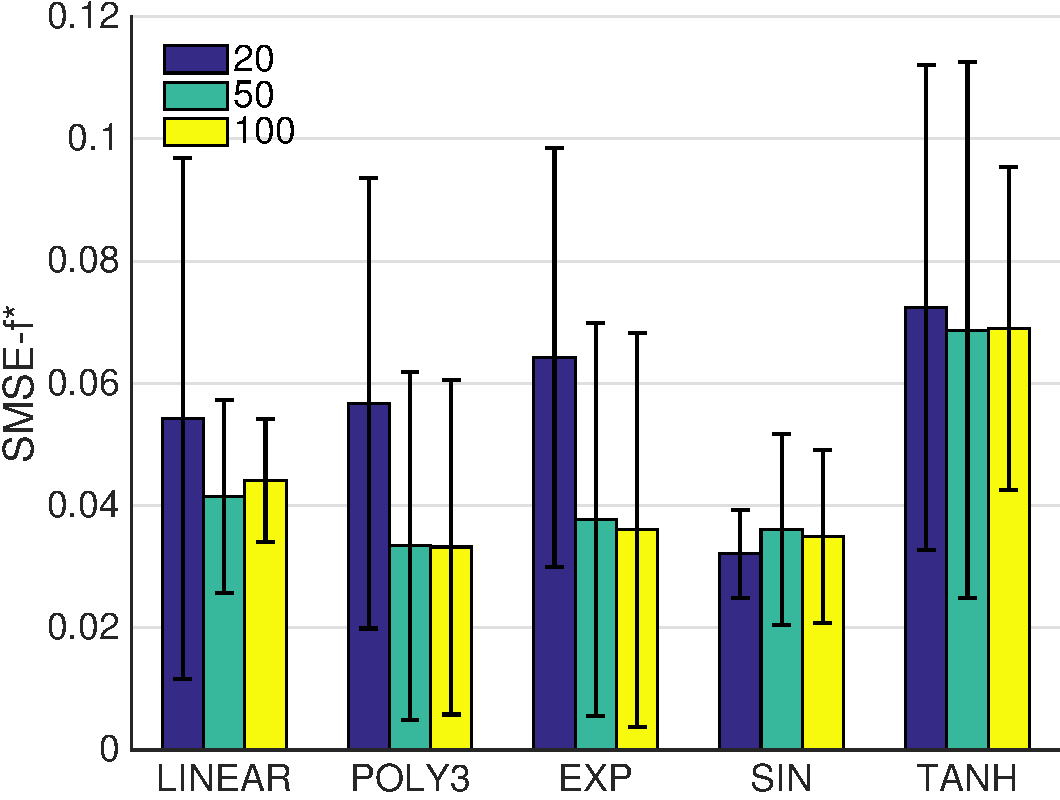
\includegraphics[width=0.31\linewidth]{toyData-EKS-SMSE-fstar} &
\includegraphics[width=0.31\linewidth]{toyData-EKS-NLPD-fstar} &
\includegraphics[width=0.31\linewidth]{toyData-EKS-SMSE-gstar} \\
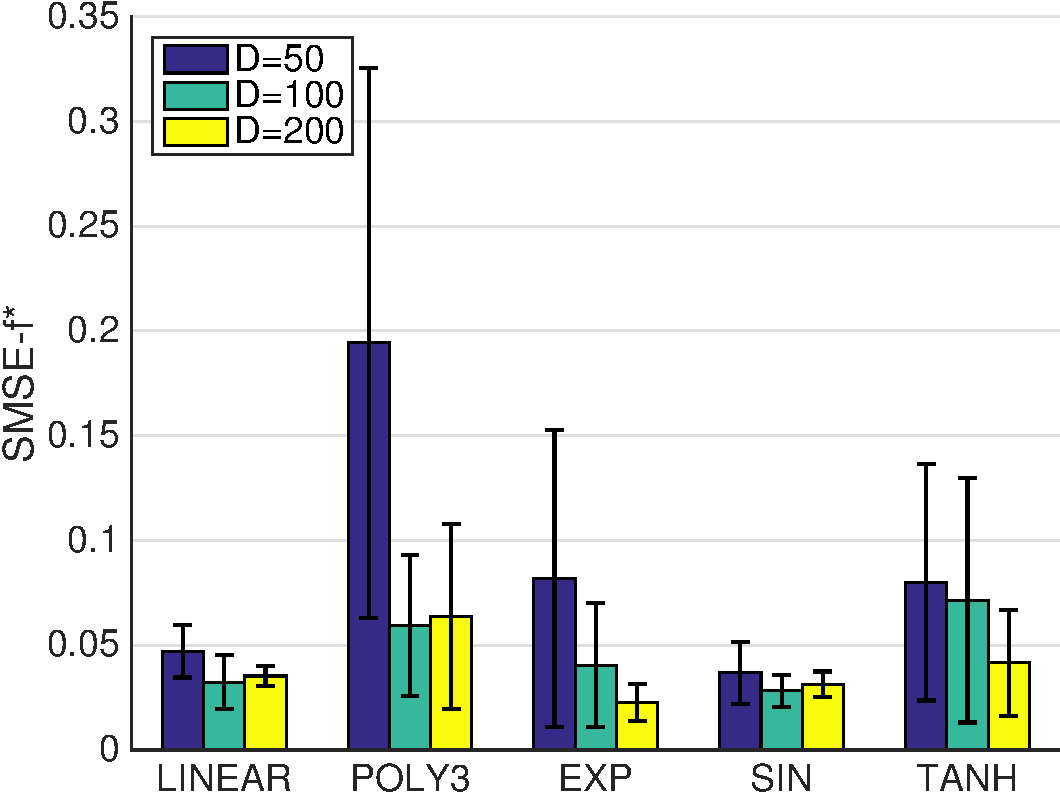
\includegraphics[width=0.31\linewidth]{toyData-UKS-SMSE-fstar} &
\includegraphics[width=0.31\linewidth]{toyData-UKS-NLPD-fstar} &
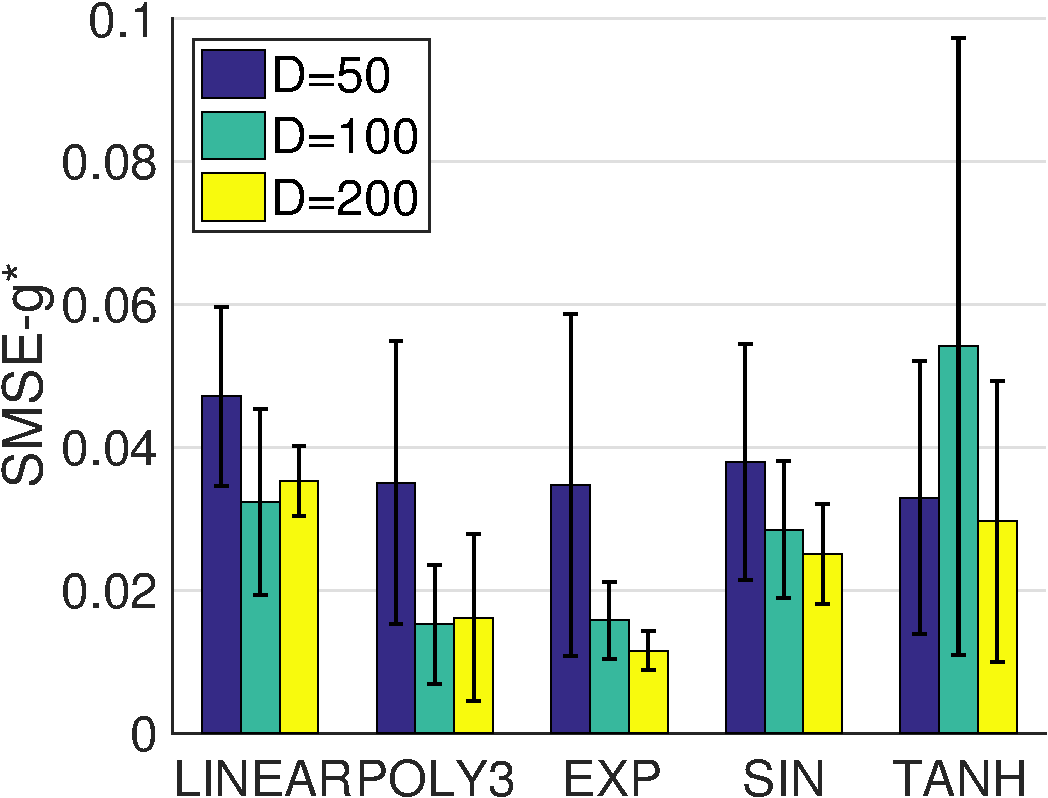
\includegraphics[width=0.31\linewidth]{toyData-UKS-SMSE-gstar} \\
\end{tabular}
\caption{The performance of the \eks (top) and \uks (bottom) as a function of the number of features used. }
\end{figure*}
%
\subsection{Binary Handwritten Digit Classification}
\begin{figure*}
\centering
\begin{tabular}{c c}
\includegraphics[width=0.45\linewidth]{uspsData-NLP}  &
\includegraphics[width=0.45\linewidth]{uspsData-ERROR-RATE}  
\end{tabular}
\caption{The performance of the \eks and \uks (bottom) on the binary classification problem for the \usps dataset as a function of 
the number of  basis used. \egp and \ugp are the original (full) \gp models.}
\end{figure*}


\subsection{Seismic Inversion}

Seismic data from the Otway basin (Pretty Hill formation) is used in this
experiment. We wish to infer the geometry and layer velocity based on seismic
reflection data, and a prior on the \emph{mean depth} of the layers (constant
mean function in a GP). There are four layers in this dataset, which means $P =
4$ (travel times) and $Q = 8$ (depth of layer boundaries, layer velocities).
Will we also need a (non-zero) prior on velocities since we have more latent
tasks than output tasks??

This can be the experimental setup;
\begin{itemize}
    \item We can validate our algorithm on 1D slices of this data (about
        100--300 interpolated seismic travel times).
    \item We will use a 1D MCMC result as `ground truth' for this problem.
    \item We need to validate on 1D because MCMC cannot optimise too many knot
        points for the splines it uses to model the geometry (dimensionality is
        too high).
    \item We can also potentially compare to the simple optimisation method
        (non-probabilistic), especially if we also need to get the gradient of
        the forward model.
    \item We can then demonstrate the \eks and \uks on the whole 2D problem,
        which is inferring a $500\times300$ grid (O(100,000) points) \emph{per
            task}. We will need an SGD/SVI implementation for this.
\end{itemize}

\section{Conclusion}

We have presented multi-task and scalable generalizations of the \egp and \ugp
algorithms introduced by \citet{steinberg-bonilla-nips-2014}, which we refer to
as \eks and \uks respectively. The \uks, like the \ugp is a `black-box' method
in that it requires no gradients of the nonlinearity in the likelihood
function in order to learn parameters/hyperparameters and perform inversions.

We have shown in our experiments that we can achieve similar prediction
performance to the original algorithms, even though we use a \rks-based
Gaussian process approximation to drastically reduce computational complexity
and increase scalability. Furthermore, we demonstrate the \eks and \uks
successfully performing a multi-task, Bayesian seismic inversion -- which is
an ideal use case for these algorithms as a fast and scalable alternative to
MCMC.

As future work we would like to use a stochastic gradient optimiser for
learning all model (hyper)parameters, and also we would like to extend the
posterior representation to a mixture of Gaussians, in a similar fashion as
\citet{nguyen-bonilla-uai-2014} and \citet{gershman-et-al-icml-12}.




\subsubsection*{References}
% A Wilson's work
 

\end{document}
